\section{El Proyecto}
El proyecto se enfoca en abordar la necesidad de utilizar los brazos robóticos SCORBOT del laboratorio CIMUBB sin la posibilidad de acceder físicamente a ellos. Ante la situación desafiante presentada por la pandemia, la solución inicial fue el uso remoto de computadoras específicas en el laboratorio para permitir la operación a distancia de las máquinas disponibles. Esta solución fue efectiva para garantizar la continuidad de las actividades educativas y de investigación en un entorno virtual, pero presentó algunas limitaciones.

Una de las principales limitaciones es la dependencia del profesor que debe estar presente físicamente en el laboratorio para realizar el monitoreo y la supervisión de la operación remota de los brazos robóticos. Esto puede ser problemático si el profesor no puede asistir al laboratorio debido a restricciones de viaje, enfermedad u otros compromisos. La falta de presencia física puede aumentar el riesgo de fallas mecánicas o incidentes inesperados, lo que podría resultar en daños considerables en el edificio o los equipos.

La idea central de este proyecto es replicar el laboratorio CIMUBB y el funcionamiento de los brazos robóticos SCORBOT de manera virtual para abordar la necesidad de impartir conocimiento sin requerir la presencialidad física en el laboratorio. Esta solución se presenta como una alternativa efectiva y sostenible ante los desafíos planteados por la pandemia y las limitaciones para acceder a los equipos en persona.

Mediante la simulación, se crea un entorno virtual que intenta recrear fielmente el laboratorio y permite a los estudiantes y profesores interactuar con los brazos robóticos SCORBOT a distancia. Esta garantiza que el conocimiento y las habilidades prácticas relacionadas con el manejo de los brazos robóticos se puedan transmitir de manera efectiva, sin incurrir en costos adicionales de equipamiento o mantenimiento de los equipos reales. Los estudiantes pueden realizar prácticas, experimentos y proyectos de manera segura y eficiente desde sus computadoras, permitiéndoles adquirir experiencia valiosa en el uso de esta tecnología sin exponerse a riesgos físicos o daños en el edificio.

Además, la simulación ofrece una ventaja significativa al permitir la flexibilidad de horarios para los profesores y estudiantes, ya que no están limitados por las restricciones de disponibilidad del laboratorio físico. Los docentes pueden impartir clases y asesorar a los estudiantes de manera remota, brindando retroalimentación y guiándolos en sus proyectos desde cualquier lugar.

\section{Otras Soluciones}
\subsection{Robocell de Intelitek}
Intelitek es una empresa dedicada a la robótica y automatización, en su pagina dicen "brindamos a las instituciones educativas entornos interactivos de aprendizaje tecnológico". 

Uno de esos entornos es el software Robocell, un software que le agrega un entorno 3D al usuario, el el cual podrá ver un robot con dimensiones reales.
\begin{figure}[h]
\centering
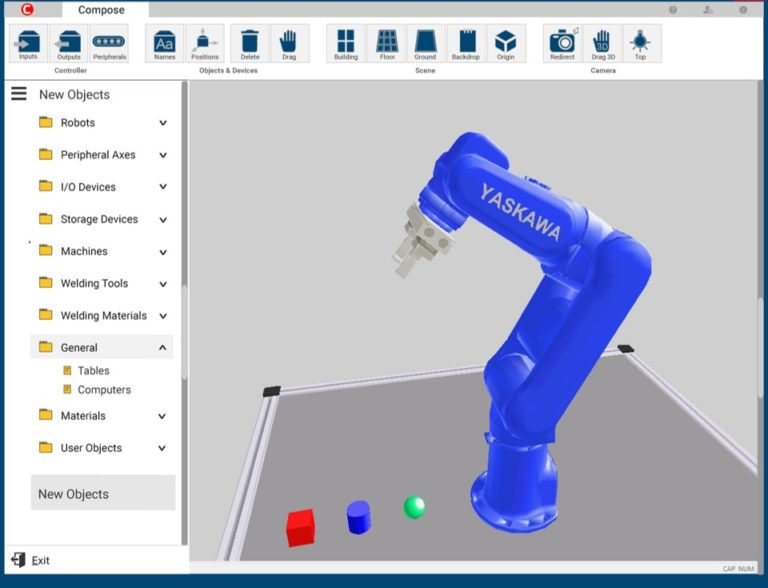
\includegraphics[width=13cm]{figures/Robocell-768x588-1.jpg}
\caption{Software Robocell}
\label{fig:robocell}
\end{figure}

En la figura ~\ref{fig:robocell} se presenta la interfaz que ofrece la empresa Intelitek, esta interfaz como tal no es util, debido que el software fue desarrollado para tener una conexión al programa Scorbase.
\clearpage 

\begin{figure}[h]
\centering
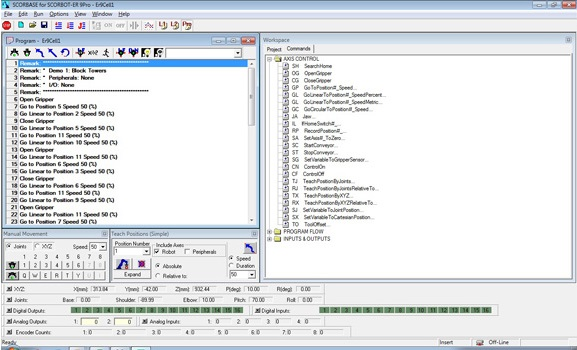
\includegraphics[width=13cm]{figures/eL_RBTC_P_ScorbaseControllerUSBPro_644x350.jpg}
\caption{Software Scorbase}
\label{fig:scorbase}
\end{figure}

En la figura ~\ref{fig:scorbase} se muestra el programa Scorbase, el cual tiene como finalidad programar y operar a los brazos robóticos, además de ofrecer soporte e integración a componentes externos, por ejemplo para realizar monitoreo o cintas transportadoras.

Este programa fue creado especialmente para la operación de maquinaria física, por lo cual carece de una opción de poder visualizar el brazo robótico en uso.

\clearpage
\begin{figure}[h]
\centering
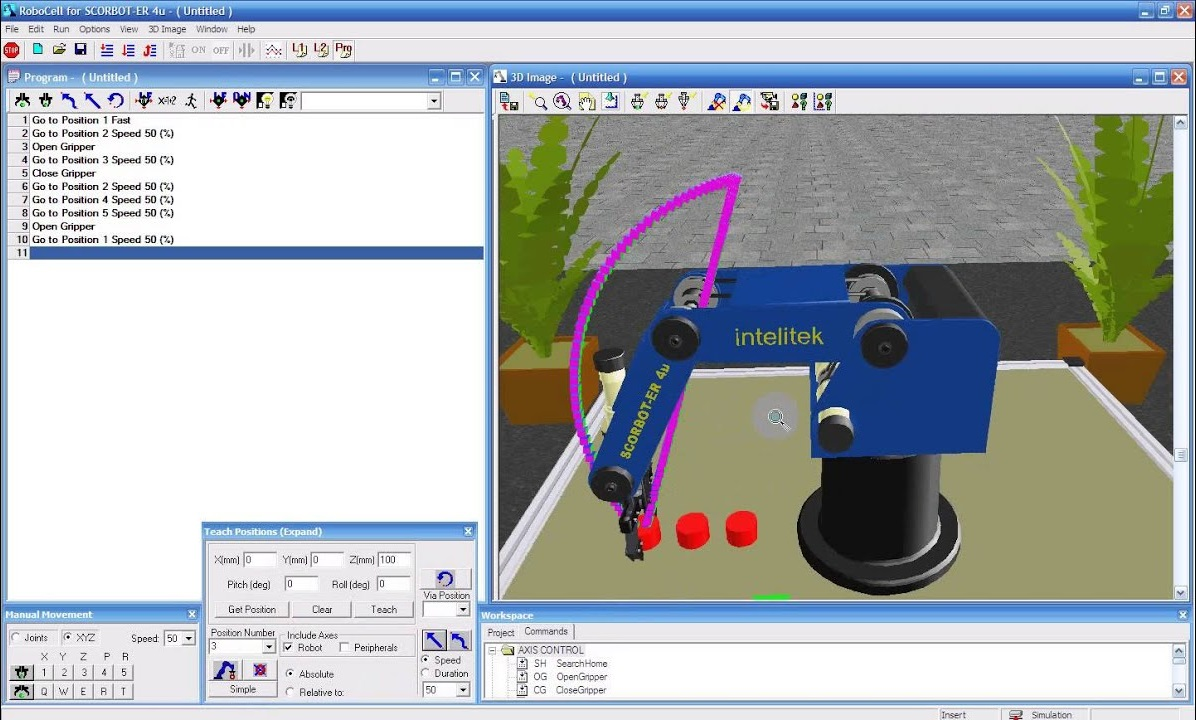
\includegraphics[width=13cm]{figures/robocell scorbase.jpg}
\caption{Software Robocell y Scorbase}
\label{fig:robobase}
\end{figure}

En la figura ~\ref{fig:robobase} se presenta ambos programas funcionando en conjunto,

\subsection{Robots Personales}

\begin{figure}[h]
\centering
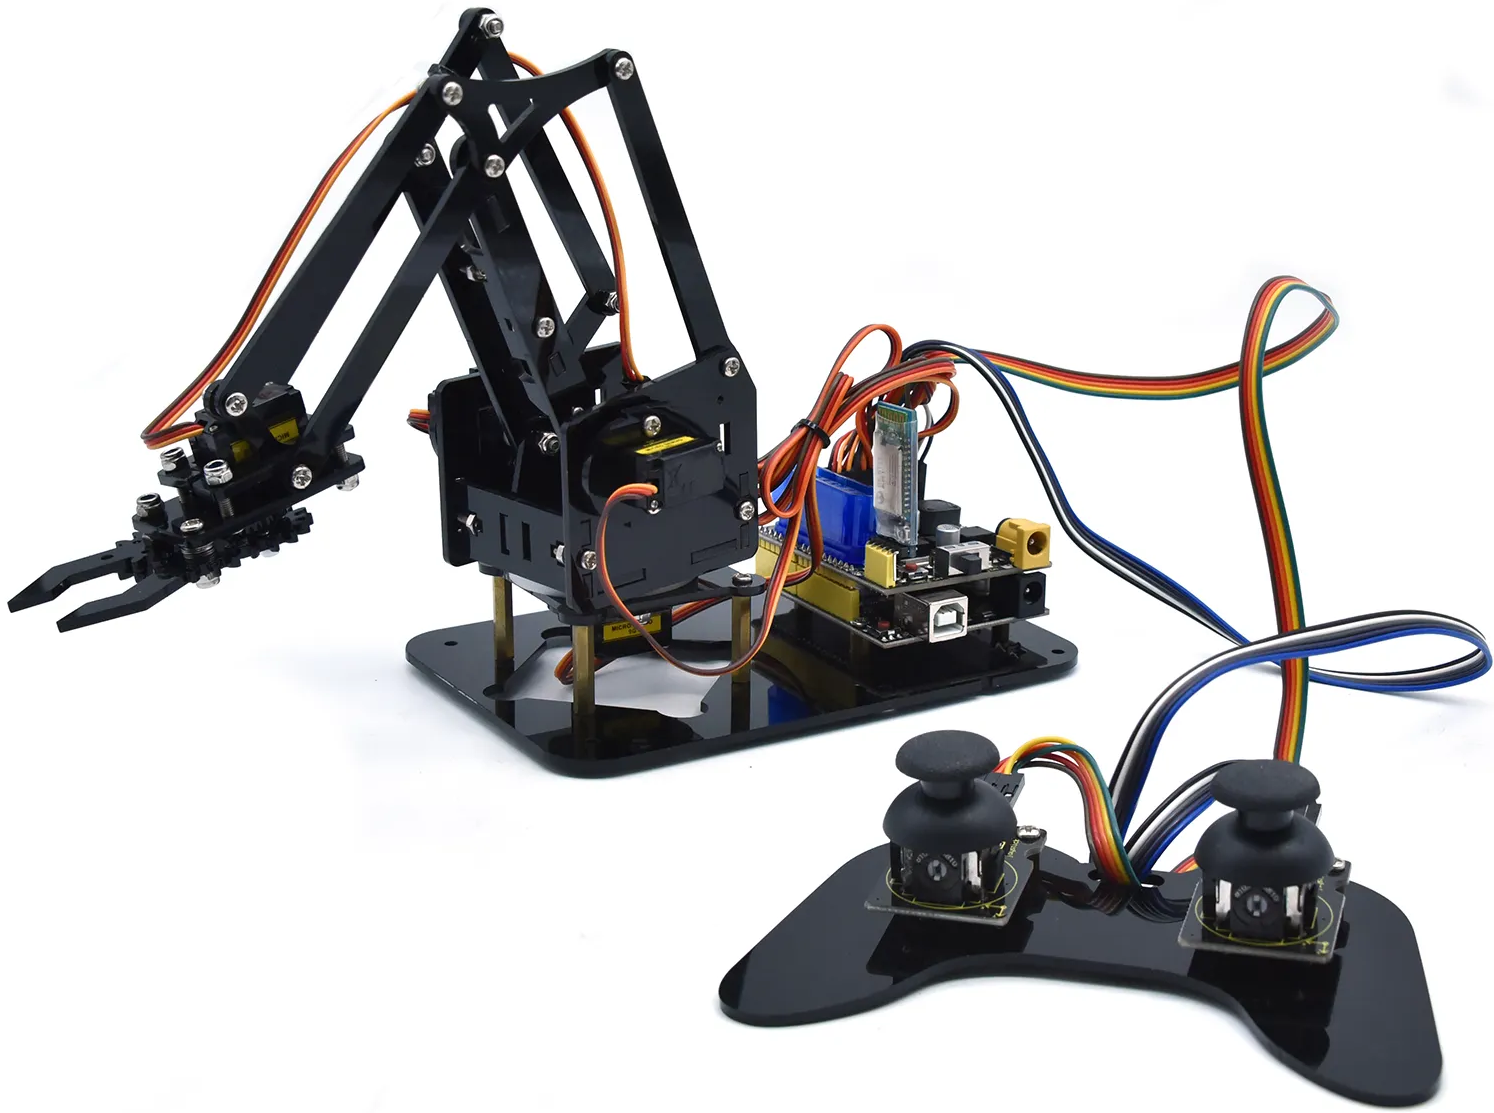
\includegraphics[width=13cm]{figures/Brazo robotico.png}
\caption{Robot Arduino}
\label{fig:robotarduino}
\end{figure}

En la figura 